\section{Overall description}
\label{sec:overall}
This section describes the software and provides a brief explanation on how the system works.

\subsection{What are Petri nets?}

Petri nets are a graphical and mathematical modelling tool for describing concurrent and distributed systems. Some examples of their applications are work flow management, embedded systems or traffic control. The main advantages of Petri nets are their graphical notation, their simplicity on the semantics, and their rich theory for analysing their behaviour. However, using the Petri net graphical notation for understanding a complex system is quite hard, and thus a user-oriented visualization is required in a way that can be understandable to users which are not necessarily familiar with Petri nets.


\begin{figure}[htp]
\begin{center}
  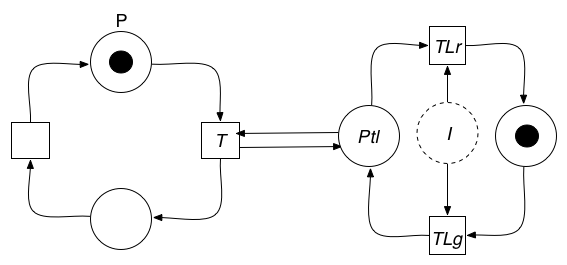
\includegraphics[width=0.8\textwidth]{image/petrinet_diagram.png}
  \caption{An example of a basic Petri net}
  \label{fig:petrinet}
\end{center}
\end{figure}

Figure \ref{fig:petrinet} presents an example of a basic Petri net. There are four different elements:

\begin{itemize}
\item Places: signified by circles, represent states.
\item Transitions: signified by squares, represent conditions.
\item Arcs: indicate which places are preconditions/postconditions for which transitions.
\item Tokens: signified by the dots, represent the elements that move in the Petri net along the places through the transitions.
\end{itemize}


Furthermore, we can see the example of \ref{fig:petrinet} as a model for a railway with a traffic light. The token in Place P represents a train moving on a railway. When this train arrives to Place P, the transition T will fire if the conditions are met. The only condition for a transition to be fired is that a token should be present on each of the incoming places of the transition.

In this scenario, the conditions are not met, as the required token in Place Ptl is missing. The visualization of this scenario would be a traffic light with a red light. If a user clicks on the Place I, it would generate a token that will turn the traffic light to green and thus the train will move.

With the aim of creating a visualization of the scenarios for the above Petri net model, an application tool is needed in order to allow the user to define where each of the elements are represented in the 3D world (geometry editor) as well as how these elements are represented (shape) and how they behave (animation). 

\subsection{Adding geometry to Petri nets}
The problem this project is tackled with is simple: We need a way to link the Petri net model to a 3D visualisation. For this purpose, once a Petri net model is created and its real life design is well-designed in the user's mind, what we call a "Geometry" is created.

For this purpose, there is a need of a geometry editor which will be used to assign a two dimensional location to the elements defined in the Petri net.

\subsection{Adding appearance to Petri net objects}
\label{sec:appearance}

Once the geometry problem is solved, a shape for each object should be defined. For instance, if places represent tracks, the shape, texture and other attributes should be linked to that object.

For this purpose, there is a need of an appearance editor which will be used to assign 3D visualization features to the elements defined in the Petri net.

\subsection{Configuration}

Before running the simulation, a definition of how the previous models are connected is needed. This is done in the configuration step as well as the validity check for the Petri net's connections to the geometry. 

\subsection{Simulating Petri nets}
The next step in visualizing Petri nets is add descriptive visuals. With the information provided by the Petri net, geometry and appearance as defined in the configuration file, the simulation is set up.

\begin{figure}[htp]
\begin{center}
  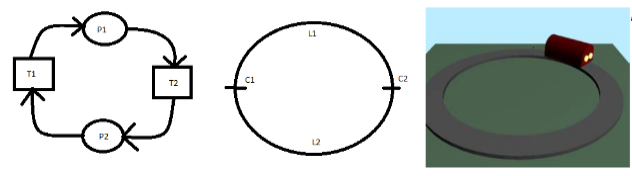
\includegraphics[width=0.8\textwidth]{image/3steps.png}
  \caption{Left: a simple Petri net.  Center: a geometry model. Right: A 3D visualization.}
  \label{fig:3steps}
\end{center}
\end{figure}

Using 3D models, textures and animations, the Petri net becomes easier to understand for the user. Continuing with the railway example, tokens become trains that move on tracks, which are places. As the tokens move from place to place, the train is animated in the 3D visualization along the tracks.

Figure \ref{fig:3steps}  shows how a simple 3D simulation of a train track and a train is made out of Petri net model and a simple geometry. Place P1 references L1 as its geometry and also has the shape of a track. The token on place P1 has the shape of a train and it moves with an animation defined by the place P1.